\documentclass[12pt,a4paper]{article}
\usepackage[utf8]{inputenc}
\usepackage[english]{babel}
\usepackage{amsmath}
\usepackage{amsfonts}
\usepackage{amssymb}
\usepackage{graphicx}
\usepackage{epstopdf}

\usepackage{fullpage}

\usepackage{float}

\begin{document}
\section{RRT}
Rapidly exploring random tree (RRT) is an algorithm builds a random tree of possible moves.
Each branch is build by extending in a random direction. 
The branch distance is forwardly being referred to as epsilon.
The RRT-Connect is a method which builds two trees, one from the goal position and one from the start position.
The first possible path that connects the two is then used.
In this report, the effect of epsilon will be investigated to find the optimal path.
As any result is a viable path, the path length is used as a way to measure the quality of the path, meaning a longer path is undesirable as it takes more time to move the robot.

\section{Pathplanning using RRT in RobWorks}
For this project, the RRT planner in RobWorks was used.
Here the path was planned from and to the two given configurations $q_{pick}$ and $q_{place}$ in the given scene.
In order to optimize the epsilon of the path planner, this was tested with respect to the time it takes to compute the path and path travelled by the tool frame.

To find a solution the path planner must be able to find a path within 15 seconds.
From figure \ref{fig:successfulVSepsilon} it can be seen that a low epsilon decreases the chances of finding a valid path.
Each path has been evaluated for collisions and a solution which caused a collision has been removed.
It is expected that a small epsilon will cause the timing to increase as it takes more small steps to reach the goal and too large steps will lead to more collisions and increase timing.
The timing and distance has been removed for those trials which did not provide a valid solution.

\begin{figure}[H]
\centering
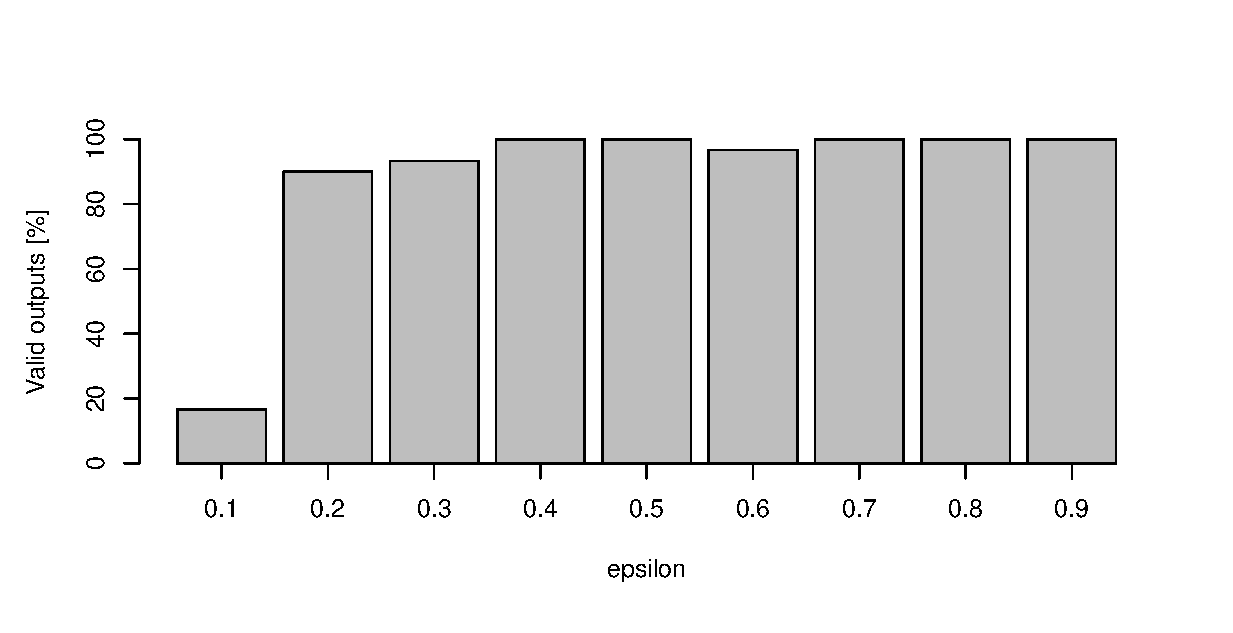
\includegraphics[width=0.7\textwidth]{../statistics/successfulVSepsilon}
\caption{figure of successful attempts within the 15 second time limit vs epsilon}
\label{fig:successfulVSepsilon}
\end{figure}

Since the RRT planner is a probabilistic approach to finding a path between the two configurations, then the path was computed 30 times.
The data gathered for the timing of the algorithm can be seen in figure \ref{fig:timeVSepsilon}.
The distance travelled by the tool in figure \ref{fig:distVSepsilon}.

\begin{figure}[H]
\centering
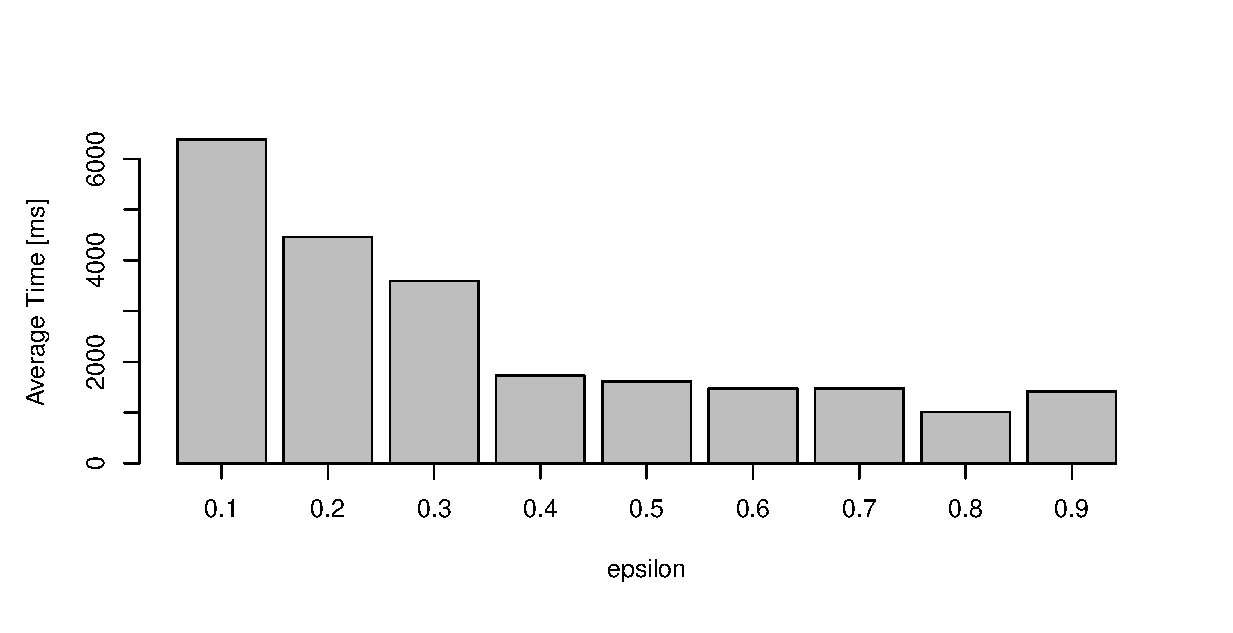
\includegraphics[width=0.7\textwidth]{../statistics/timeVSepsilon}
\caption{figure of time vs epsilon}
\label{fig:timeVSepsilon}
\end{figure}


\begin{figure}[H]
\centering
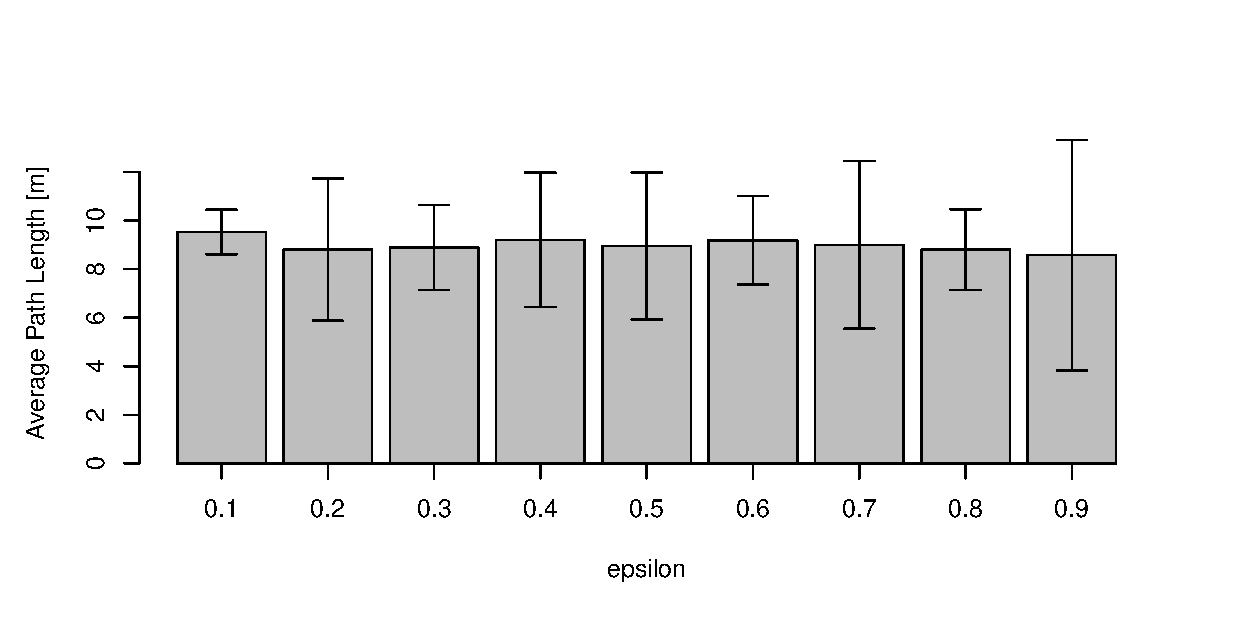
\includegraphics[width=0.7\textwidth]{../statistics/distVSepsilon}
\caption{figure of tool-frame path length vs epsilon}
\label{fig:distVSepsilon}
\end{figure}


It can be seen on the figures the, passing an epsilon of 0.5, then the likelihood of finding a path within 15 seconds is close to 100\%.
Furthermore the average time is only around two seconds when a epsilon of 0.5 is used.

Considering the path length of the tool, then they all fall between 8 and 10 meters, but with some having a deviation of four meters.

In this scenario an epsilon of 0.8 is advised since it both has a fast computation time and the path length is not deviating too much around its average.

\end{document}